\chapter{The 5 Multi-s}%
\label{cha:multi_5}

This chapter is simply a conglomeration of multiple usage possibilities.

\section{Multi-Camera / Mixer}%
\label{sec:multicamera_mixer}

Use the Mixer Viewer to see multiple media playing simultaneously in re-sizable mini-viewers.  This can be used in various ways and is useful to edit videos shot by multiple cameras from different viewpoints that were simultaneously recorded in order to create a single good video.  Everything will have to be initially synced so you can decide which one of the camera angles is best suited at any time. 

The number of cameras/mixers you can have is generally limited to the available resources on your computer.  Currently, the number of File Descriptors available in the OS limits cameras to about 50.  If you have many \textit{mixer viewers} you will probably want to use proxy mode whenever possible.  Also, in the \texttt{Settings $\rightarrow$ Playback A} tab \textit{Video Out} section, uncheck \texttt{play every frame} and choosing a Video Driver of \texttt{X11} with \texttt{use direct X11 render if possible} checked, will provide better performance.

Figure~\ref{fig:multicam01} shows 9 media sources in the left corner, the composed video in the right corner, the timeline with the top video track with pieces of the 9 overwrites, and the choice in Resources of Mixed.

\begin{figure}[htpb]
    \centering
    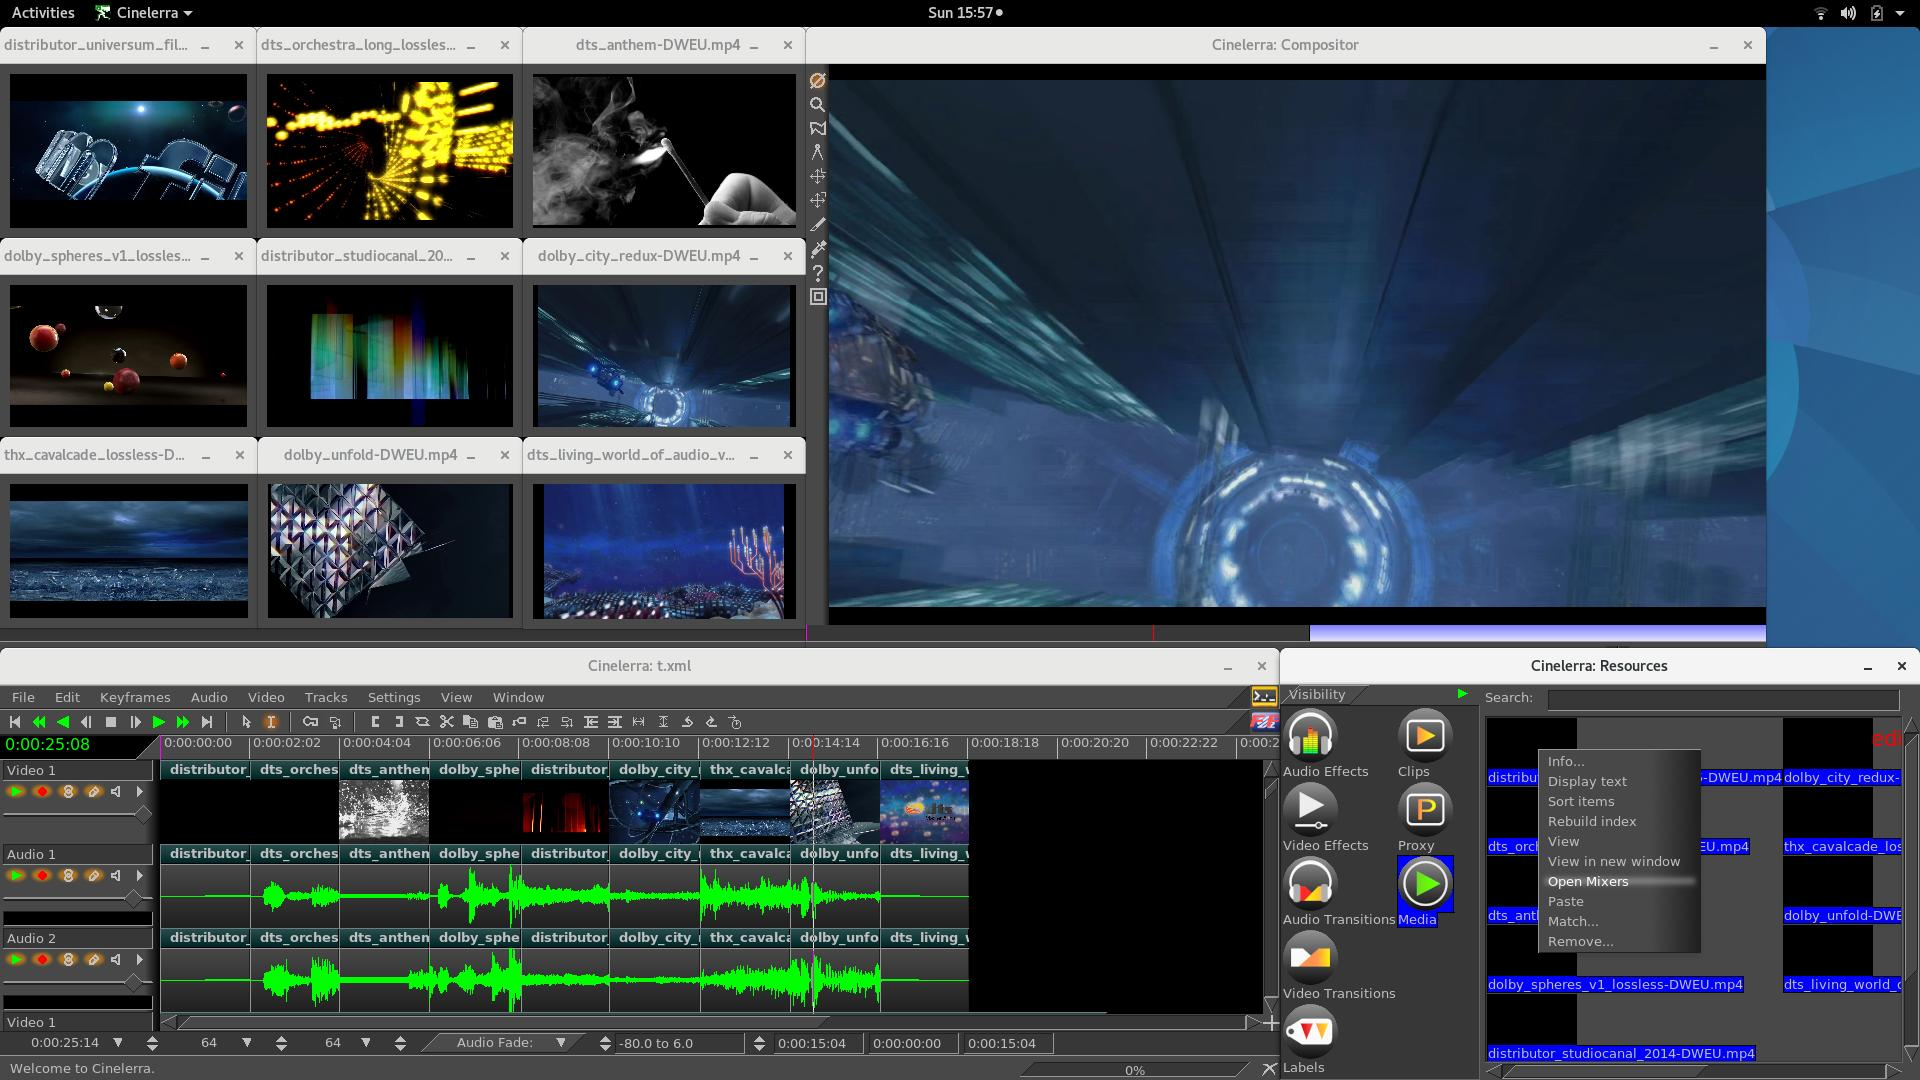
\includegraphics[width=0.9\linewidth]{images/multicam01.png}
    \caption{Using Mixer capability in Cin for multiple cameras}
    \label{fig:multicam01}
\end{figure}

\subsubsection*{Easiest Method to Getting Started}%
\label{ssub:easiest_method_started}

\begin{enumerate}
    \item This method assumes all of your media or cameras are aligned the way you want them already.
    \item From the \textit{File} pulldown, create a \texttt{New project} with the desired format for Audio and Video output (or you can just use the default).
    \item \texttt{File $\rightarrow$ Load} the media files you want to work with using \textit{Create new resources only}.
    \item In the Resources window, with  the Media folder, highlight the list of media you want to \textit{Mix}. This is done using a ctrl or shift mouse button press as you would in a standard listbox selection.
    \item Right click the mouse on the media selection and choose \texttt{open mixers}. This opens multiple mixer viewer windows, one for each media item that was highlighted.  You can
    do them 1 at a time instead.  This also adds the source media tracks to the main window.
    \item Now use the timeline to play and you will see all viewers/cameras playing.  Stop when you get to the
    end of the \textit{good} camera playback.
    \item Simply double click the \textit{good} mixer viewer and from where you first started playing to the playback insertion pointer is the source section, which will be pasted in the destination video/audio tracks at the top of the new project.
    \item Repeat steps 6-7.  Start playing again, stop when you want, double click the desired mini-viewer!
\end{enumerate}

\subsubsection*{Some Hints and Caveats}%
\label{ssub:hints_caveats}

\begin{itemize}
    \item You can easily overwrite a section of the new track by \textit{selecting} a section on the timeline, then double click on one of the mini-viewers to overwrite/replace that section.
    \item If you edit the output tracks, it only edits output tracks, and the input tracks may no longer be lined up.
    \item You can add a silent section by selecting past a section and start overwriting that section from then on.
    \item If you use the cursor hairline to create the selection endpoint, it must be past the end of the destination.
    \item The compositor shows composed media.  This is the media that will be rendered.
    \item The program always uses overwrite as the paste operation.
    \item Use the timeline edit handles to move the start and end points of that section.
    \item Only middle mouse drag handle operations should be used normally.
    \item Other drags will displace the media source/destination timeline correspondence.
    \item To re-tile the mixer windows after you have resized and moved them around, you can use the Window
    pulldown of \texttt{Tile mixers} or the shortcut of \texttt{Alt-t}.
\end{itemize}

\subsubsection*{But, I want to use only the first set of audio tracks\dots}%
\label{ssub:but_use_only_first_audio}

There are many cases where you may want to compose using media from several different tracks while using the the same audio tracks as associated from a specific viewer.  Since mixer source tracks can be updated any time by using a mixer toggle, this makes it possible to do this.  

Procedure to update the mixer audio source track list:

\begin{enumerate}
    \item Single click to highlight the mixer window you want to re-associate to the audio track.
    \item In that audio track’s patchbay click the expand toggle, the arrow on the right side.
    \item In the expanded pane that appears, there is another arrow on the left side.  This icon has the tooltip \textit{Mixer}.  Click this and because in step \#1 you highlighted the mixer window, it will now be toggled on.  Once you click the mixer icon it will then point up.
    \item Now, disassociate any audio that is unwanted by expanding its patchbay and toggling off the mixer.
\end{enumerate}

\subsubsection*{Expert Usage}%
\label{ssub:expert_usage}

When you double click a mixer viewer window, it operates an \textit{overwrite} paste operation.  This moves \textit{src} (source) track edits to \textit{dst} (destination) track edits over the same selected timeline region.

\begin{itemize}[noitemsep]
    \item \textit{Src tracks} should be not playable and not armed in the main window patchbay gui.
    \item \textit{Dst tracks} should be playable and armed in the main window patchbay gui.
\end{itemize}

Each mixer viewer maintains a list of the tracks which will be used as src. This list is made visible selecting the window with the left mouse button.  When the mixer viewer is selected, a highlight is drawn around the media image.  All track patchbay \textit{mixer} toggles are updated to reflect the src tracks included in the selected viewer src track list. The track patchbay toggles can be used to manage the list.

\begin{itemize}[noitemsep]
    \item \textit{Turning on} a toggle (pointing up) includes the track in the src track list.
    \item \textit{Turning off} a toggle (pointing right) removes the track from the src track list.
\end{itemize}

New Mixer viewers can be created using the main menu \texttt{Window $\rightarrow$ Mixer Viewer}, or with a shortcut of \texttt{Shift-M}.  When a new viewer is created, the currently enabled patchbay \textit{mixer} toggles are used to create the viewer source track list.  The toggles are cleared after the window is created.  This is to improve the work flow.  Use the following list of steps to create individual mixer viewers.

To create a list of mixer viewers:

\begin{enumerate}
    \item Setup the session \texttt{settings $\rightarrow$ format}, width, height, frame rate, color model, aspect ratio.
    \item Create dst tracks using the a/v track pulldowns (or use shortcuts \texttt{‘t’} / \texttt{‘T’}),  armed and playable.
    \item Append src tracks using \texttt{file $\rightarrow$ open $\rightarrow$ append tracks}, or the resource window using pasting.
    \item Using the track patchbay, disarm editing and disable playback of the audio/video src tracks.
    \item Using the track patchbay, mark the new tracks as \textit{mixer} source to be added to the viewer.
    \item Create a mixer viewer using the main menu pulldown, or the shift "\texttt{M}” shortcut.
    \item Repeat steps $3-6$ for each mixer viewer needed for the session editing.
\end{enumerate}

When you single click a mixer window, it becomes selected and highlighted and all of the patchbay mixer toggles are updated to reflect the state of the viewer’s src tracks.  Tracks that will be src are shown as enabled.  If you change a toggle, the src tracks for the selected window will be modified.  This means you can associate or dis-associate any media track to any mixer window.

When you double click a mixer window, an overwrite paste is invoked.  The mixer viewer’s src tracks are overwritten to the dst tracks.  The timeline region for both the source and destination are the same for the overwrite paste function.  The selection region is used if it is active.  If the selection is empty, that is it is a hairline, the selection region is from the end of the destination playable edits to the selection cursor hairline.  The hairline must be past the end of the playable edits on the destination tracks.

The mixer viewer configuration is saved with the session data.  When a saved session is loaded in \textit{replace project} or \textit{replace project and concatenate tracks}, the mixer viewer will be reopened.

\subsubsection*{Using Proxy with \textit{Open Mixers}}%
\label{ssub:using_proxy_open_mixers}

The best way to use proxy with your multiple cameras is to follow the steps below:

\begin{enumerate}
    \item Load media with insertion strategy of \texttt{create resources only}.
    \item Highlight the media in the Resources window and right click on this to choose \textit{open mixers}.
    \item Use the \textit{Settings} pulldown and choose  \texttt{Proxy settings\dots} to bring up the proxy menu.
    \item Choose the size and other options you want and click the checkmark \texttt{OK}. If you choose the option \texttt{Beep when done} you will hear a short beep if all media is already proxied or a longer beep when all proxies have been created.
    \item When your editing is complete, use \textit{Settings} pulldown and proxy to \texttt{original size}.
\end{enumerate}

Instead of Open Mixers, you can Insert Mixers with new tracks at the timeline insertion point.

\subsection{Mixer Align by Audio}%
\label{sub:mixer_align_audio}

Multi-camera footage of a single event can have various shots starting and ending at different times. So when the footage start times are different, you can use the mixer audio to synchronize the clips on the timeline. The program algorithm attempts to find and align automatically the waveforms of the media.

Synchronizing multiple camera videos based on audio tracks can be done with Cinelerra-GG easily enough with the Window pulldown Mixers… → Align mixers option.  Align mixers brings up a window displaying your mixers, the currently selected Master Track, and a list of all of the Audio Tracks (figure~\ref{fig:mixer-align01}).  There is a limit of 32 audio tracks per each mixer (that should be enough!)

\begin{figure}[htpb]
    \centering
    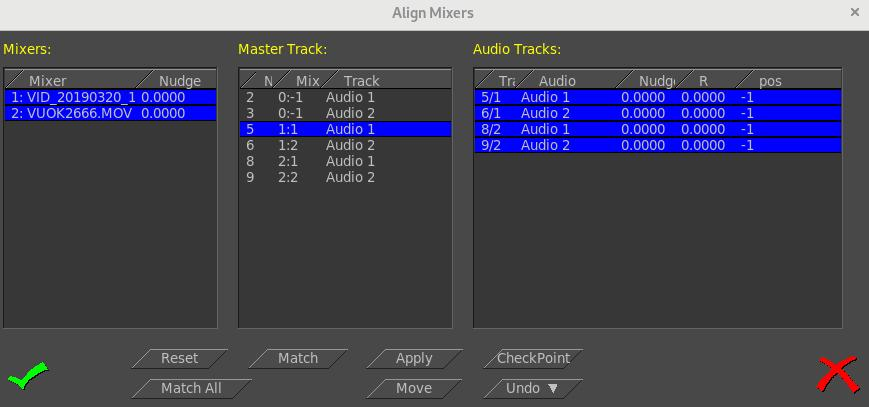
\includegraphics[width=0.9\linewidth]{images/mixer-align01.png}
    \caption{Align Mixers window}
    \label{fig:mixer-align01}
\end{figure}

Two different methods of aligning the audio for mixers are available. They are most easily referred to by the button that is pressed --- \texttt{Match} and \texttt{Match All}. There are also 2 methods of activating the alignment --- \texttt{Apply} and \texttt{Move}.  

\textit{Match} consists usually of the next set of steps to take advantage of this feature:

\begin{enumerate}
    \item Load your camera media with insertion strategy of \textit{resources only}
    \item Highlight in the Resources window, all of the media you want to mix.
    \item Right mouse button on one of the media and click on Open Mixers; all mixer windows come up.
    \item Provide a small target audio pattern on the Master Track for syncing by marking with the In/Out points ([ and ]).
    \item Make a selection on the timeline in which to look for the pattern. Left mouse click, then drag select and highlight a search time domain.
    \item Use the Window pulldown, \texttt{Mixers\dots $\rightarrow$ Align mixers} to bring up its dialog window.
    \item Highlight in the first listbox, the Mixer number you want to align. Click on \texttt{Match}. This will take a few seconds so watch the rendering time percentage on the lower right hand side zoom panel. The buttons will be ghosted out until finished. Now note the changed values in the Audio Tracks listbox.
    \item If you are satisfied with the calculated Nudge values -- that is they are very close to $1.0$ -- in the Audio Tracks listbox and the audio track selected as the Master Track in the Master Track listbox, hit the \texttt{Apply} button.
    \item If you plan on performing more alignment tasks, click on Checkpoint so you can go back to a previous step in case you make a mistake.
    \item Last, click on the \texttt{OK green} checkmark or to cancel click on the \texttt{red X}.  Or just close the gui.
\end{enumerate}

\paragraph{Reset} is used to start over with the current session data, not an undo.  This means you can use the match repeatedly to refine alignments.  All of the Audio Tracks listbox values will be reset.

\paragraph{Checkpoint} provides a method to create checkpoints that save the current state.  This is especially helpful while learning or doing more complicated operations where you might make a mistake or do not like the results and need to get back to a previous state.

\paragraph{Undo} is used to put the media back to a previous state on the timeline.  If you choose \textit{start over} the session will reload with the original, before any changes were applied.  You can also go back to any of your previous checkpoints that you created earlier which are listed there, such as \texttt{chkpt 1}.

\paragraph{Match All}is used when you have several mixers, instead of only picking 1 to match, it picks the best match for EACH of the mixer tracks based on a single master track. So when you hit Apply, each track might move differently. You do not set In/Out points but you have to make a selection within which to match.

\paragraph{Apply} button will apply the nudges that were generated during the Match or Match All execution (figure~\ref{fig:mixer-align02}).

\paragraph{Move} is very handy when you are using mixers, if you have an edit somewhere that you need to fix specifically without moving any of the other track pieces. In this case you have to select a section (like you do a group, but do not make a group), generate a match, and then you can just \textit{Move} that set only - everything else stays where it is at its current location (figure~\ref{fig:mixer-align03}).

\begin{figure}[htpb]
    \centering
    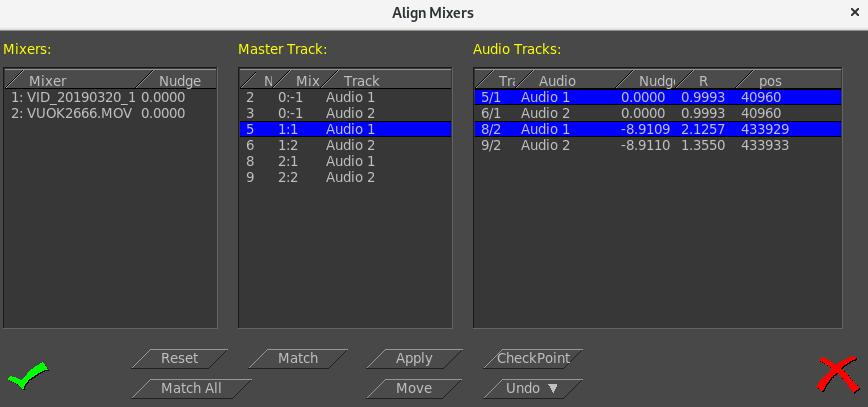
\includegraphics[width=0.9\linewidth]{images/mixer-align02.png}
    \caption{Aligned mixer window after "Match". Note the Nudge amounts above.}
    \label{fig:mixer-align02}
\end{figure}

More detailed information follows about how this all works and the information in the dialog window.  It is important to know that the result of the calculation is \textit{best match} but you can still override the selections if you decide there is a better one.  The dialog window is split into 3 sections:

\begin{enumerate}
    \item \textit{Mixers} lists the mixers that are active by highlighting them all initially. You can decide that you do
    not want 1 or more mixers to be used in the correlation calculation by un-highlighting the one(s) that should not be used. In some cases you have to have at least 2 in order to align audio.
    \item \textit{Master Track} lists each of the audio tracks currently loaded for all of the mixers. You can decide to highlight a different audio track to be used as the master for correlation, but only 1 can be used.
    \item \textit{Audio Tracks} lists each of the mixer audio tracks.  Again, you can highlight a different set of which
    mixer audio tracks that you want to use for the waveform correlation.  Any audio tracks that are not
    highlighted, that is \textit{turned off}, will not be considered in the correlation calculation.
\end{enumerate}

\begin{figure}[htpb]
    \centering
    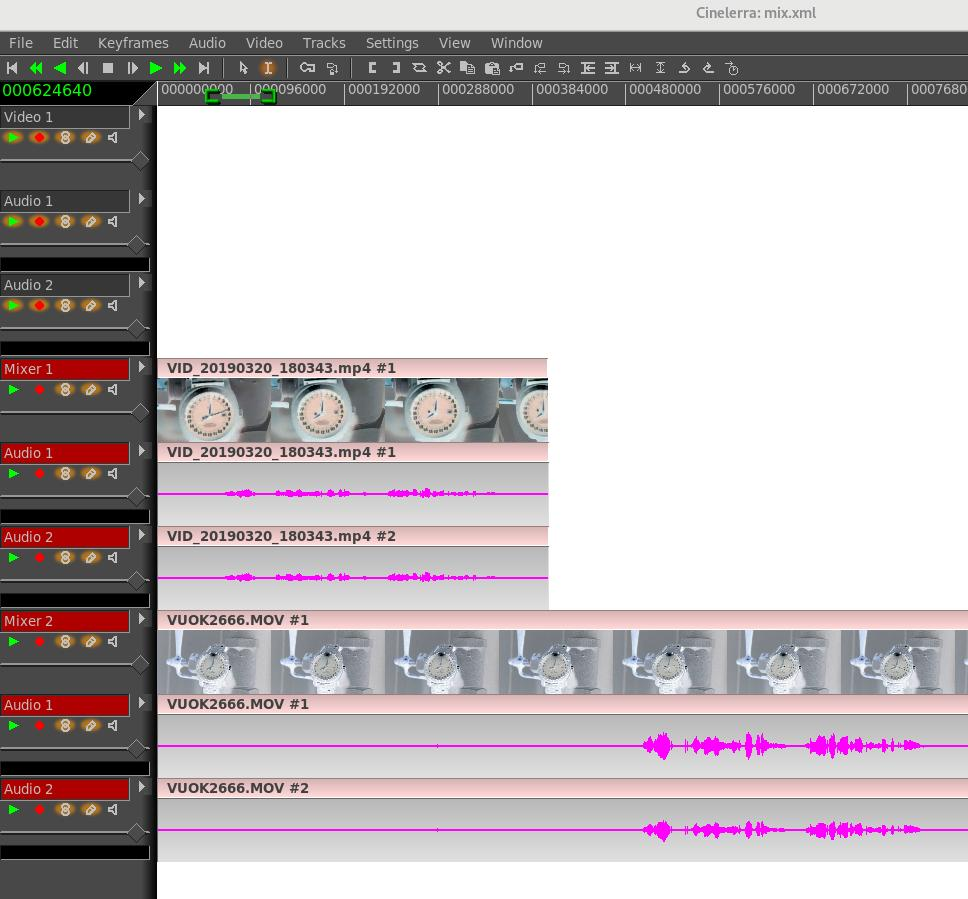
\includegraphics[width=0.9\linewidth]{images/mixer-align03.png}
    \caption{Match setup for aligning by audio.  Note that [ ] are set over a sample waveform highlighted selection that includes that.}
    \label{fig:mixer-align03}
\end{figure}

The corresponding input position is determined by track input correlation.

The letter \textit{R} in the Audio Tracks listbox represents the correlation value.  "R=1.0" designates that if both the pattern and the matching section were in the highlighted area, they are completely correlated -- this is a good self-test to check.
$Nudge=0.0$ means just that.

The header \textit{pos} stands for the timeline position. When the \texttt{Apply} button is pressed, only the Mixers listbox is relevant at that time.

The Mixer with the master track generally does not move, everything else will be lined up (figure~\ref{fig:mixer-align04}).

\begin{figure}[htpb]
    \centering
    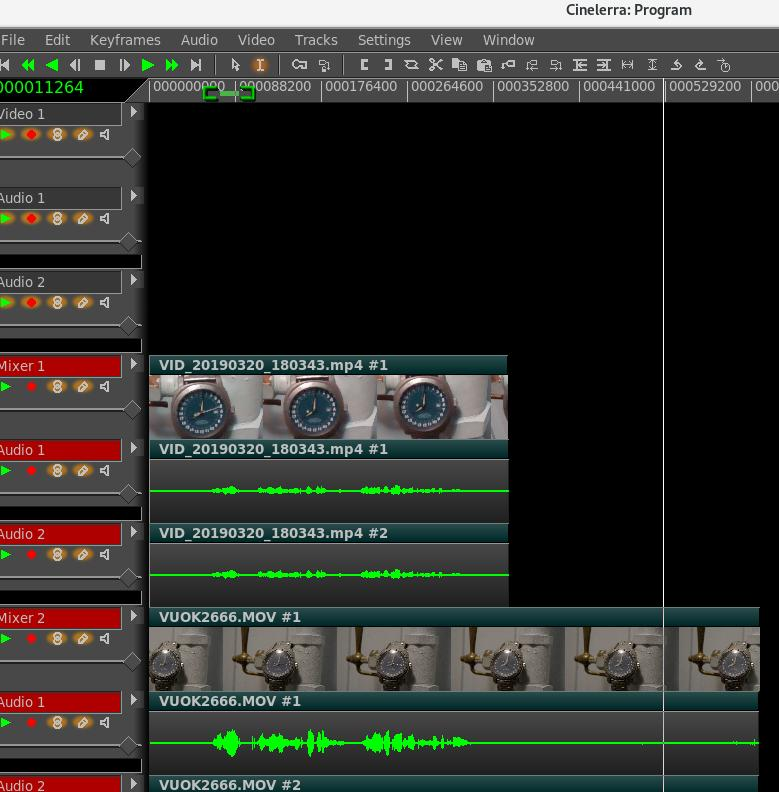
\includegraphics[width=0.9\linewidth]{images/mixer-align04.png}
    \caption{An audio Match is complete. Note the waveform is aligned.}
    \label{fig:mixer-align04}
\end{figure}

\textit{Match All} option basically consists of the following steps:

\begin{enumerate}
    \item Highlight the Mixer to use in the Mixer listbox.
    \item Highlight the Master Track you want to use in the Master Track listbox.
    \item On the timeline, mark your selection on the Master Track.
    \item Click on the \texttt{Match All} button.
    \item Note the nudge values to see if they make sense, and if so, press \texttt{Apply}.
\end{enumerate}

\textit{Match} option basic steps (just for comparison with Match All):

\begin{enumerate}
    \item Set the In/Out points [ ] of the target.
    \item On the timeline, mark your selection.
    \item Click on the \texttt{Match} button.
    \item Note the nudge values to see if they make sense, then press \texttt{Apply} (or \texttt{Move} when doing a group).
\end{enumerate}

\subsection{Recover Mixer Windows}%
\label{sub:recover_mixer_windows}

\begin{wrapfigure}[14]{O}{0.4\linewidth} 
    \vspace{-8ex}
    \centering
    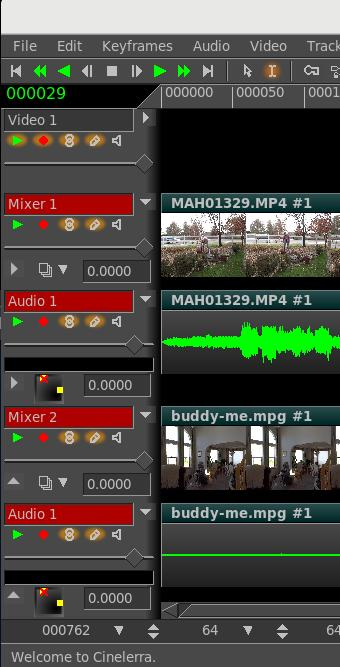
\includegraphics[width=0.7\linewidth]{images/mixer-patchbay01.png}
    \caption{Mixer  patchbay}
    \label{fig:mixer-patchbay01}
\end{wrapfigure} 

It is a hazard that you might accidentally \textit{undo} (\texttt{z}) too far and lose your mixer windows.  Here are the steps to recover.  It is recommended that you make a backup of your project before performing the recovery steps just in case there are other problems.

In the patchbay box to the left of the main timeline, there is a right pointing arrow on the right side.  This is called the \textit{Expander} (figure~\ref{fig:mixer-patchbay01}).  When you click on each expander, another line appears below that expander arrow and the timeline track height is slightly increased.  If you \texttt{Shift-click} on a single expander, the patchbay will expand for all of the tracks.

\begin{enumerate}
    \item Expand all of the patchbay lines, either one by one, or Shift-click on one to do them all. This is so you can see the \textit{mixer} right pointing arrow on the second expanded line.
    \item Use the Window pulldown and choose \textit{Mixer Viewer} to bring up a new mixer window.  Now you will be making an association between the mixer viewer and the track’s video.
    \item Click on the new mixer window to make sure it is highlighted with a white border. This designates it as the \textit{in use} mixer viewer.
    \item Set your play to the beginning of the video using the \texttt{Home} key or \texttt{Home} transport button.
    \item In the patchbay for a video track click on the \textit{mixer} arrow on the expanded $2^{nd}$ line which is a right facing arrow.  Now the arrow will point up.  If there are audio tracks with that video, click on each of its audio tracks \textit{mixer} arrow until they point up also.
    \item Next move your insertion pointer on the timeline where there is video.  Some of the time this just helps so that the new mixer viewer window gets redrawn and you can see that the images appear; but the image may not appear until the program does a redraw later.  Now the mixer viewer should be
    correctly associated.  Note if you have large video, give it some time to update.  You may have to click on the mixer viewer window if the image does not show.  You can always start over with that mixer if you encountered any problems.
    \item Click the arrows that are pointing up in that video and its audio so they go back to pointing right. That mixer viewer is complete so you need to do this to make sure the \textit{mixer} arrows are off.
\end{enumerate}

Repeat steps 2 through 7 for each of the mixer viewers you need going down the patchbay starting on step 2 first with Mixer 1, then 2 to 7 steps for Mixer 2, then again run 2 to 7 for Mixer 3 and so on.

Sometimes the association does not stick initially.  If not, highlight the mixer viewer with the problem, change the mixer arrows to point up, and reassociate.

\section{Multi-Pane Support}%
\label{sec:multipane_support}

The main Cinelerra edit window holds the Track Canvas which can be divided into 4 panes of track data: 1 or 2 vertical panes and/or 1 or 2 horizontal panes.  To split the track, use the Window pulldown, and then click on \texttt{Split X} or \texttt{Split Y} depending on how you wish to split the track.  Alternatively, the canvas pane types can be changed using keys \texttt{<Ctrl-1>} for toggle split horizontal or \texttt{<Ctrl-2>} for toggle split vertical.  Or the track can be split into panes by using the \texttt{+ widget} in the lower right hand corner of the track canvas.  Once the track has been divided, you can use the + widget shortcut or the drag bars to change the size of the panes.

Multi-Pane, or split screen, allows you to look at the first part of a movie at the same time as a part that is a long ways away on the timeline which would have been off the screen.  By having multiple panes, you can see the 2 parts you want to look at simultaneously and drag/drop easily between the 2.  Also, the \textit{X pane split} is extremely convenient for laptop users and computer monitors with small screens since it can be used with horizontal scrolling with the \texttt{mouse wheel + Ctrl}.  The \textit{Y-pane split} makes it easy to see 2 simultaneous drag and drop zones when you have lots of tracks (figure~\ref{fig:multi-pane01}).

\begin{figure}[htpb]
    \centering
    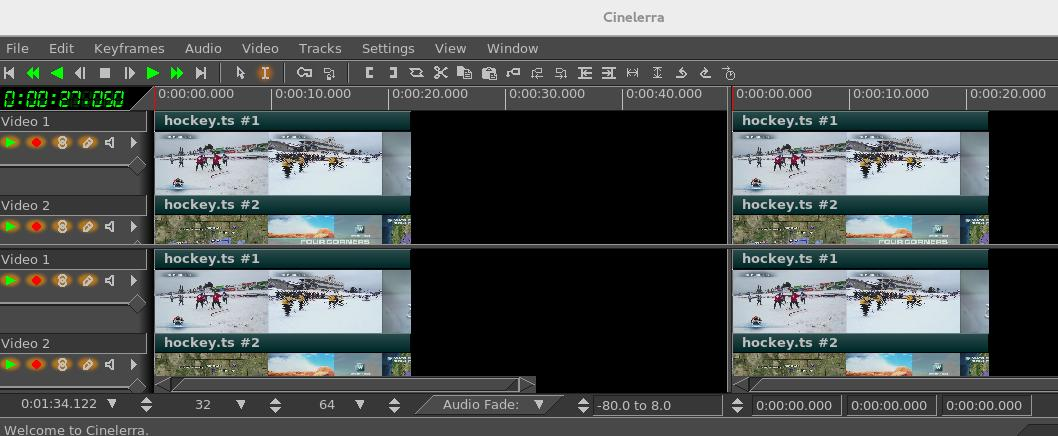
\includegraphics[width=0.9\linewidth]{images/multi-pane01.png}
    \caption{Shown are 4 panes that have split the main track canvas for some editing scenarios}
    \label{fig:multi-pane01}
\end{figure}

\section{Multi-screen / Playback Configuration}%
\label{sec:multiscreen_playback_configuaration}

Cinelerra-GG supports 2 separate preferences for the playback configuration.  Cinelerra can be operated in a single or dual screen configuration, both by using Xinerama or dual screen configuration of X windows.  It will take some setup using Xconfig to make this work.

The \texttt{Settings $\rightarrow$ Preferences} menu has \textit{Playback A and Playback B} tabs.  The target display and audio device configuration can be separate, to support up to 2 display and/or audio device stations.  The active configuration displays an asterisk (*) in its selection tab and the selected tab will be made active when \texttt{OK} is pressed.  For example: you may have a dual screen monitor system with the left screen showing the cinelerra main window and the right screen showing the composer.  Another setup might use a monitor for the left screen and an HDTV as the right screen displaying the composer.  When a playback configuration is selected, the audio/video device configuration is switched to the playback selection.  The active playback setup can be changed through use of the menu pulldown of \texttt{Settings $\rightarrow$ Preferences} or via the remote control menu selection (see the section Remote Control for DVB for more detail). 

\subsubsection*{Yes, you can watch TV on cinelerra instead of cinelerra on TV.}%
\label{ssub:watch_tv_on_cinelerra}

Figure~\ref{fig:multi-screen01} shows partial window of \textit{*Playback A} selected and the second tab for \textit{Playback B}.  Note that on the bottom right of the window, \texttt{Default B Display:} is set to $:0.1$, representing the setting for Screen 1.  On the unseen \textit{Playback A} window, the \texttt{Default A Display:} will be set to $:0.0$ meaning for Screen 0.  Otherwise, the default would be nothing there or just <empty>.

\begin{figure}[htpb]
    \centering
    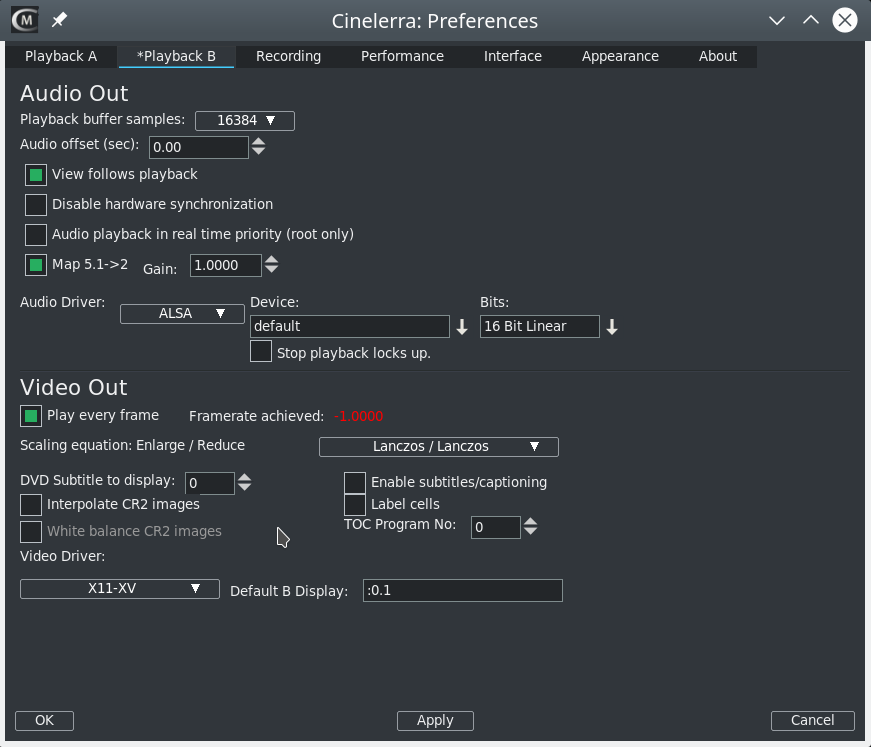
\includegraphics[width=0.8\linewidth]{images/multi-screen01.png}
    \caption{Multi-screen Playback example useful for watching Cinelerra run on the \textit{big screen}}
    \label{fig:multi-screen01}
\end{figure}

\section{Multi-Session}%
\label{sec:multi_session}

You can run as many sessions of Cinelerra as your computer resources allow.  However, if you are using the same \texttt{\$HOME/.bcast5}, changes you make for one may impact the others. You can always create and rename a new .bcast5 from:
\texttt{Settings $\rightarrow$ Preferences $\rightarrow$ Interface $\rightarrow$ Index files: $\rightarrow$ Index files go here:}

\section{Multi-Viewer Window Support}%
\label{sec:multi_viewer_window_support}

You can create as many Viewer windows as you want in Cinelerra.  These are handy for users who are adept at working with a lot of different clips simultaneously.  By bringing up multiple Viewer windows, each clip can be edited in its own area, making it easy to see all of the separate pieces.  After you have loaded some media files, to start another Viewer window, right click on one of the pieces of media in the Resources window.  This brings up a menu of several options, one of which is \texttt{view in new window}.  Choose this option and that media will come up in a new Viewer window for you to work (figure~\ref{fig:multi-view01}).

\begin{figure}[htpb]
    \centering
    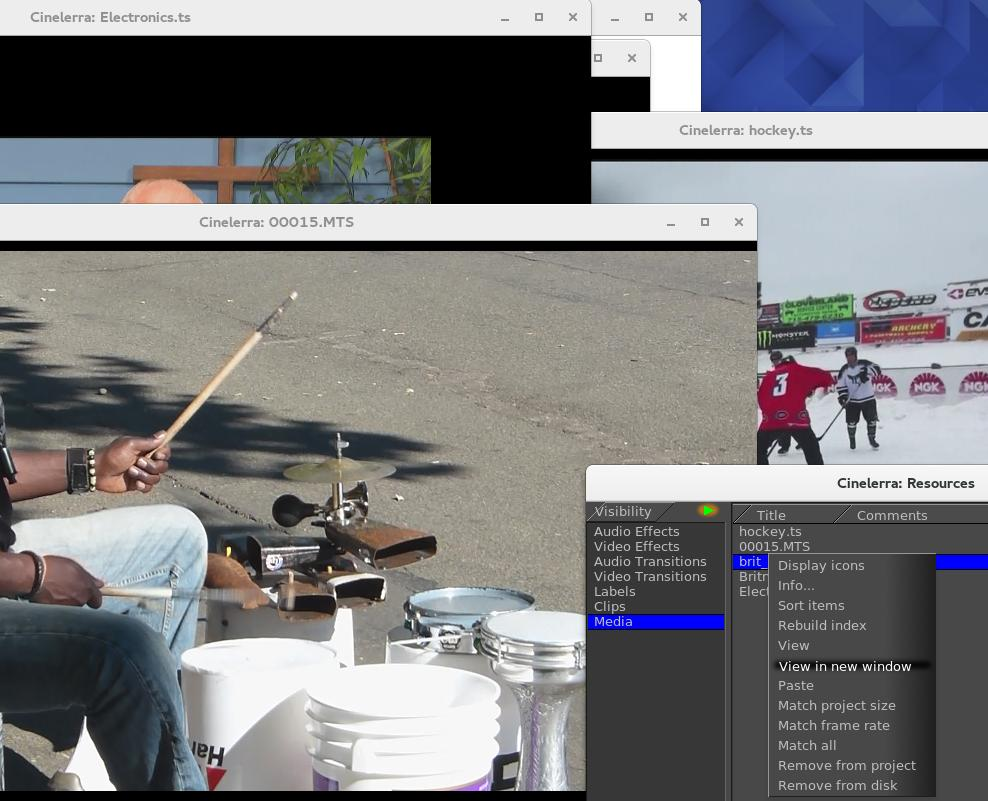
\includegraphics[width=0.8\linewidth]{images/multi-view01.png}
    \caption{Shown here are 3 Viewer windows and the \textit{View in new window} popup}
    \label{fig:multi-view01}
\end{figure}

